\documentclass[border=10pt]{standalone}

\usepackage{tikz}
\usepackage{tikzsymbols}
\usetikzlibrary{calc,patterns,shapes.geometric}

\def\centerarc[#1](#2)(#3:#4:#5){\draw[#1] ($(#2)+({#5*cos(#3)},{#5*sin(#3)})$) arc (#3:#4:#5);}

\begin{document}
	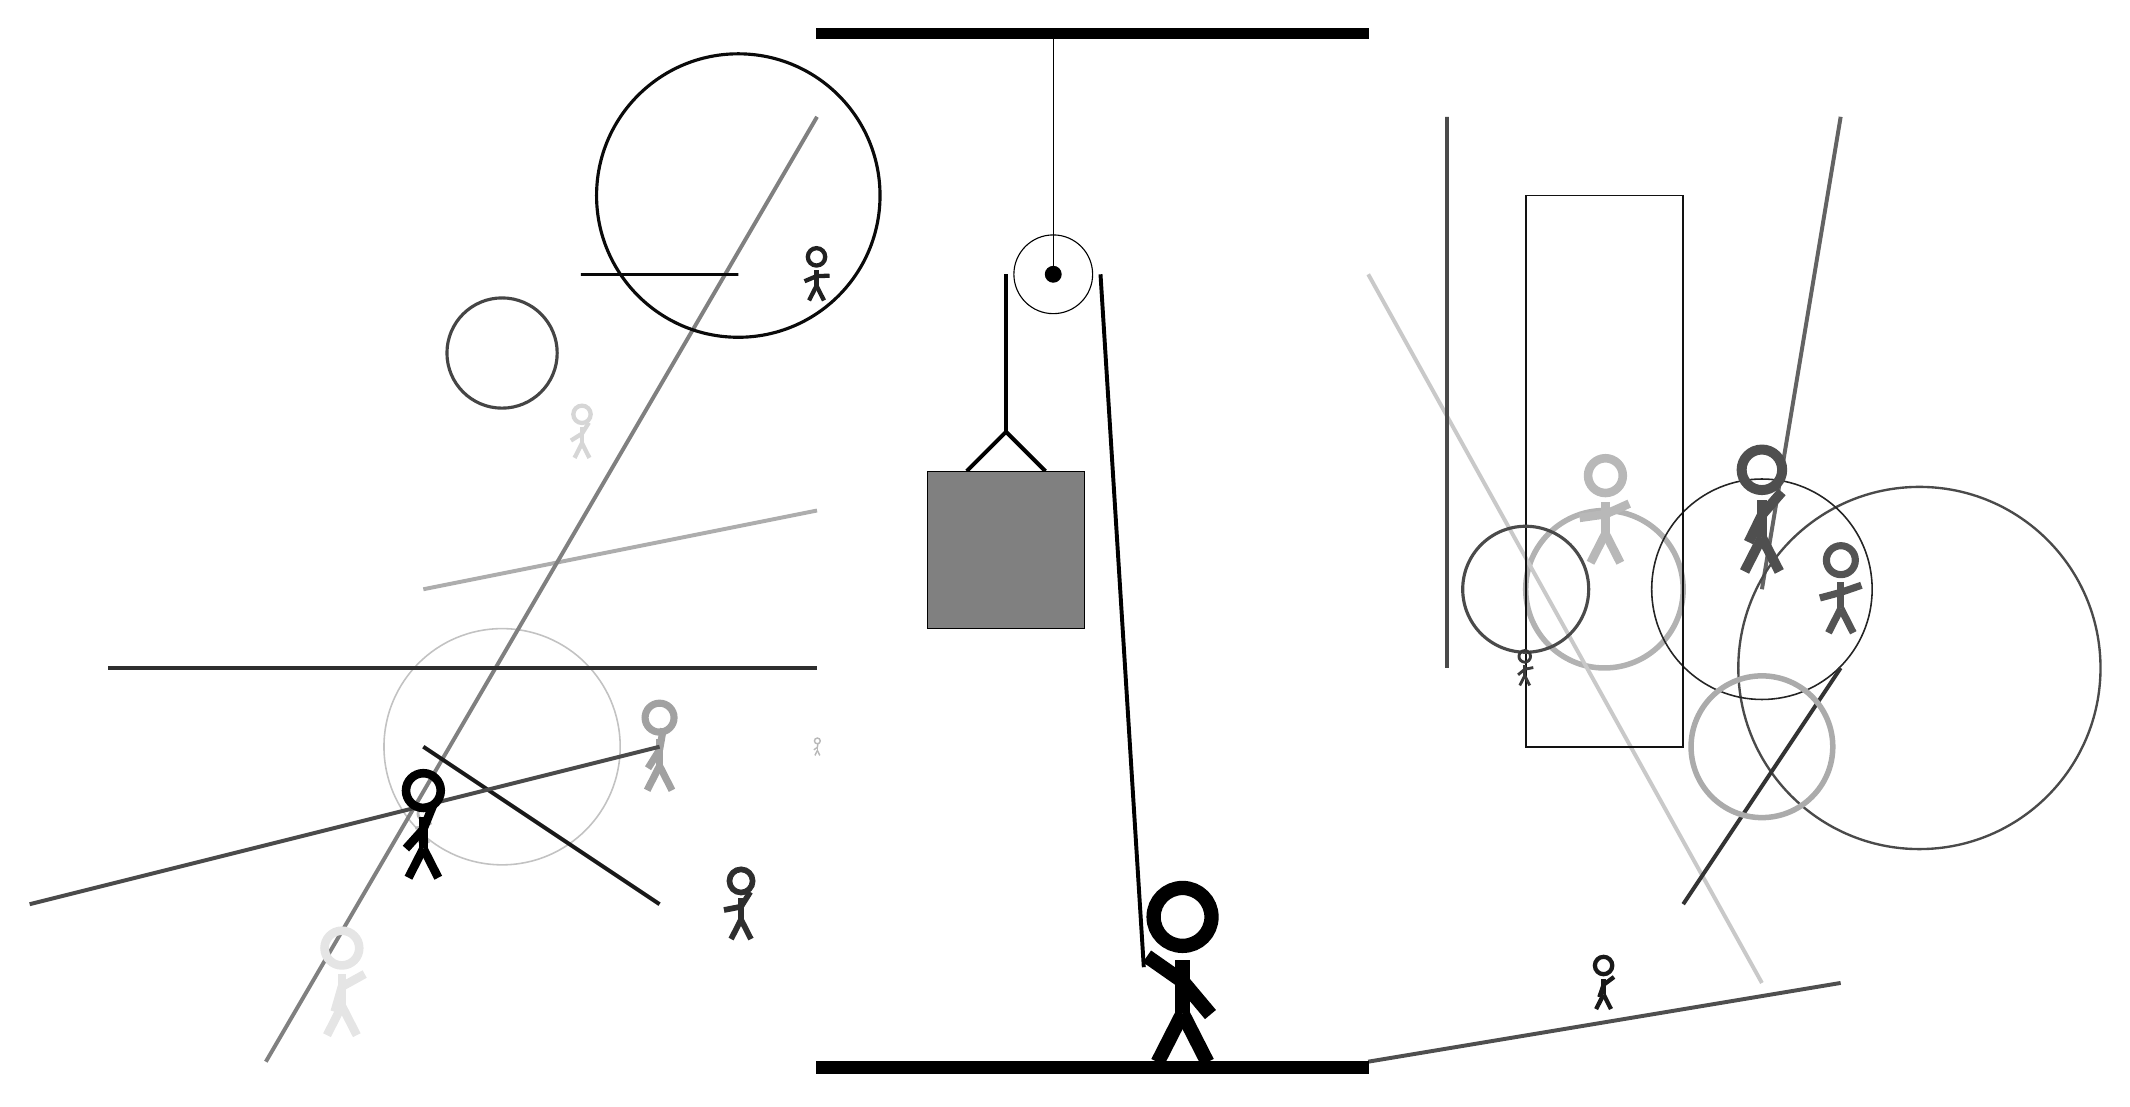
\begin{tikzpicture}
		%%%%% START %%%%%
		
		\draw[fill=black] (-2, 10) rectangle (5, 10.125);
		
		\draw (1, 7) circle (0.5);
		\draw[fill=black] (1, 7) circle (0.1);
		\draw (1, 10) -- (1, 7);
		
		\draw[line width=0.5mm] (-0.1, 4.5) -- (0.4, 5.0) -- (0.9, 4.5);
		\draw[fill=black!50] (-0.6, 4.5) rectangle (1.4, 2.5);
		
		\draw[line width=0.5mm] (0.4, 7) -- (0.4, 5.0);
		\centerarc[line width=0.5mm](1, 7)(0:180:0.6);
		\draw[line width=0.5mm](1.6, 7) -- (2.15, -1.8);
		
		\node at (2.6, -1.9) {\Strichmaxerl[10][-35][-50]};
		
		\draw[line width=0.5mm, color=black!69](5, -3) -- (11, -2);
		
		\node[line width=0.7mm, color=black!82] at (-3, -1) {\Strichmaxerl[4][11][58]};
		\node[line width=0.4mm, color=black!37] at (-4, 1) {\Strichmaxerl[5][58][80]};
		\draw [line width=0.7mm, color=black!30](8, 3) circle (1.0);
		\draw[line width=0.5mm, color=black!21](10, -2) -- (5, 7);
		
		\draw [line width=0.2mm, color=black!24](-6, 1) circle (1.5);
		\draw[line width=0.5mm, color=black!61](10, 3) -- (11, 9);
		
		\draw[line width=0.5mm, color=black!32](-7, 3) -- (-2, 4);
		\node[line width=0.3mm, color=black!16] at (-5, 5) {\Strichmaxerl[3][32][58]};
		\draw[line width=0.5mm, color=black!50](-2, 9) -- (-9, -3);
		\draw [line width=0.3mm, color=black!71](12, 2) circle (2.3);
		\node[line width=0.5mm, color=black!10] at (-8, -2) {\Strichmaxerl[6][74][29]};
		\node[line width=0.6mm, color=black!28] at (8, 4) {\Strichmaxerl[6][8][24]};
		\draw[line width=0.5mm, color=black!82](-2, 2) -- (-11, 2);
		\node[line width=0.3mm, color=black!90] at (8, -2) {\Strichmaxerl[3][71][37]};
		\node[line width=0.6mm, color=black!87] at (-2, 7) {\Strichmaxerl[3][23][2]};
		
		\draw[line width=0.4mm, color=black!97] (-3, 7) rectangle (-5, 7);
		
		\draw [line width=0.2mm, color=black!86](10, 3) circle (1.4);
		\node[line width=0.3mm, color=black!28] at (-2, 1) {\Strichmaxerl[1][35][82]};
		\draw[line width=0.2mm, color=black!93] (7, 8) rectangle (9, 1);
		\node[line width=0.2mm, color=black!28] at (-7, 0) {\Strichmaxerl[2][9][27]};
		
		\node[line width=0.7mm, color=black!67] at (11, 3) {\Strichmaxerl[5][15][19]};
		\draw[line width=0.5mm, color=black!80](9, -1) -- (11, 2);
		\draw[line width=0.6mm, color=black!77] (-4, 4) rectangle (-4, 4);
		\draw [line width=0.7mm, color=black!33](10, 1) circle (0.9);
		\draw[line width=0.5mm, color=black!90](-4, -1) -- (-7, 1);
		\draw [line width=0.4mm, color=black!71](7, 3) circle (0.8);
		\node[line width=0.2mm, color=black!77] at (7, 2) {\Strichmaxerl[2][40][11]};
		
		\draw[line width=0.5mm, color=black!71](-4, 1) -- (-12, -1);
		
		\node[line width=0.6mm, color=black!69] at (10, 4) {\Strichmaxerl[7][64][49]};
		\draw [line width=0.4mm, color=black!96](-3, 8) circle (1.8);
		
		\node[line width=0.3mm, color=black!100] at (-7, 0) {\Strichmaxerl[6][48][68]};
		\draw[line width=0.6mm, color=black!71] (6, 2) rectangle (6, 9);
		\draw [line width=0.4mm, color=black!73](-6, 6) circle (0.7);
		
		\draw[fill=black] (-2, -3) rectangle (5, -3.15);
		
		%%%%% END %%%%%
	\end{tikzpicture}
\end{document}